% !TEX program = xelatex
% 논문 USV_swarm_defense_EAAI_KR_real §4.2 "적 무리 군집화" 식 (1)~(4) 해설 자료.
% 도판·수치는 make_figs.py 가 figs/ 에 생성한다 (numbers.json 참조).
\documentclass[11pt,a4paper]{article}
\usepackage{kotex}
\usepackage{fontspec}
\setmainfont{TeX Gyre Termes}[Ligatures=TeX]
\setmainhangulfont{HCR Batang}[AutoFakeBold=2.0, AutoFakeSlant=0.2]
\setsanshangulfont{HCR Dotum}[AutoFakeBold=2.0, AutoFakeSlant=0.2]
\usepackage{amsmath, amssymb}
\usepackage{graphicx}
\usepackage{booktabs, array, multirow}
\usepackage{xcolor}
\usepackage[margin=22mm]{geometry}
\usepackage{caption}
\usepackage{float}
\usepackage{tcolorbox}
\usepackage[hidelinks]{hyperref}
\graphicspath{{figs/}}
\setlength{\parskip}{4pt}
\setlength{\parindent}{0pt}
\linespread{1.15}
\captionsetup{font=small, labelfont=bf}
\renewcommand{\figurename}{그림}
\renewcommand{\tablename}{표}
\usepackage{tabularx}
\definecolor{navy}{HTML}{1F3A5F}
\definecolor{keybg}{HTML}{EEF3FA}
\definecolor{whybg}{HTML}{FFF6E5}
\newtcolorbox{keybox}[1][핵심]{colback=keybg, colframe=navy, title=#1, fonttitle=\bfseries, boxrule=0.6pt, left=6pt, right=6pt, top=4pt, bottom=4pt}
\newtcolorbox{whybox}[1][왜 이렇게 쓰나]{colback=whybg, colframe=orange!70!black, title=#1, fonttitle=\bfseries, boxrule=0.6pt, left=6pt, right=6pt, top=4pt, bottom=4pt}
\newcommand{\vt}{\vartheta}
\newcommand{\bfe}{\mathbf{e}}
\newcommand{\bfm}{\mathbf{m}}
\newcommand{\bfc}{\mathbf{c}}
\newcommand{\bhat}{\hat{\mathbf{b}}}
\newcommand{\dhat}{\hat{\mathbf{d}}}
\newcommand{\vapp}{v^{\mathrm{app}}}
\newcommand{\dgap}{\delta_{\mathrm{gap}}}

\title{\bfseries 적 무리 군집화 --- 식 (1)--(4) 해설\\[4pt]
\large\mdseries USV 군집 방어 원고 (\texttt{USV\_swarm\_defense\_EAAI\_KR\_real}) \S4.2 보조 자료}
\author{}
\date{2026-09-20}

\begin{document}
\maketitle
\vspace{-14pt}

\begin{keybox}[이 자료의 목적]
원고 \S4.2의 네 식은 하나의 파이프라인이다: \textbf{적선 위치} $\to$ (1)~\textbf{방위각} $\to$ (2)~\textbf{방위 사이 빈틈} $\to$ (3)~\textbf{빈틈 개수 = 무리 수} $\to$ 라벨링 $\to$ (4)~\textbf{무리 요약 4종}.
각 식을 [문제 $\to$ 직관 $\to$ 식 $\to$ 숫자 예 $\to$ 왜 이 형태인가] 순서로 풀고, 적선 5척짜리 예제 하나를 처음부터 끝까지 끌고 간다.
모든 수치는 \texttt{make\_figs.py}로 계산했고 실제 구현(\texttt{boatattack\_sim/env/clustering.py})과 대조했다(부록~A).
\end{keybox}

\begin{figure}[H]
\centering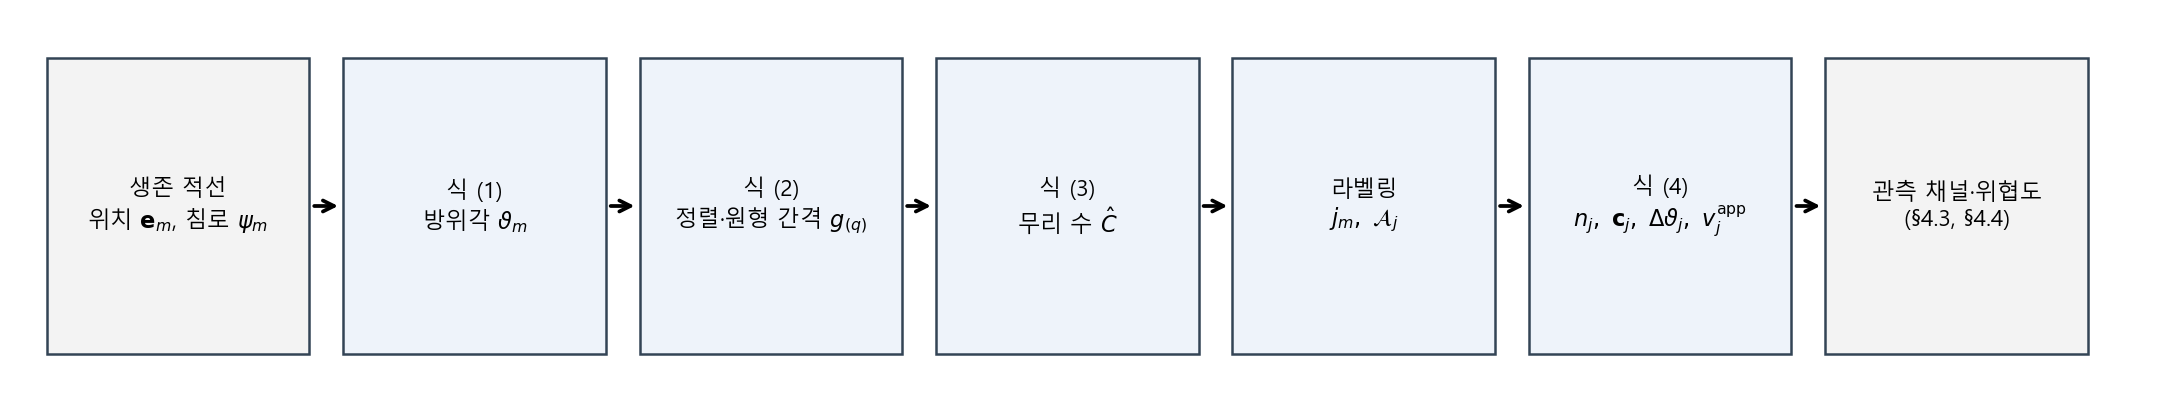
\includegraphics[width=\textwidth]{fig_pipeline.png}
\caption{군집화 파이프라인. 파란 상자가 \S4.2의 네 식과 라벨링 단계.}
\end{figure}

\section{왜 군집화가 필요한가}

원고의 두 판단 계층(그물 전개 판단, 요격점 선택)은 개별 적선이 아니라 \emph{무리}를 단위로 배정한다.
적선이 12척이든 20척이든 관측 채널은 최대 $C=4$개 무리 자리만 가지므로, 매 결정 시점마다 생존 적선을 "모선에서 봤을 때 같은 방향에서 오는 덩어리"로 묶어 4개 이하로 요약해야 한다.
이때 묶는 기준은 \textbf{모선 기준 방위각}이다. 방어 자원(그물)이 모선 주위 어느 \emph{방향}에 배치돼야 하는지가 핵심 결정이므로, 거리보다 방위가 먼저다.

\medskip
예제(이 자료 전체에서 사용): 적선 5척, 모선 기준 방위·거리·침로는 표~\ref{tab:ex}와 같다.
\begin{table}[H]
\centering\small
\caption{예제 적선 5척. 적선 번호 $m$은 시뮬레이터가 부여한 순서(정렬 전).}\label{tab:ex}
\begin{tabular}{c c c c c}
\toprule
적선 $m$ & 방위 $\vt_m$ & 거리 (m) & 위치 $\bfe_m=(x,y)$ (m) & 침로 $\psi_m$ \\
\midrule
1 & $200^\circ$ & 5000 & $(-1710,\,-4698)$ & $20^\circ$ \\
2 & $10^\circ$  & 4200 & $(729,\,4136)$    & $190^\circ$ \\
3 & $210^\circ$ & 5200 & $(-2600,\,-4503)$ & $60^\circ$ \\
4 & $30^\circ$  & 4400 & $(2200,\,3811)$   & $215^\circ$ \\
5 & $20^\circ$  & 4000 & $(1368,\,3759)$   & $200^\circ$ \\
\bottomrule
\end{tabular}
\end{table}
모선 $\bfm=(0,0)$, 적선 속력 $v_e = 10$ m/s, 무리 상한 $C=4$, 간격 임계 $\dgap = 12^\circ$ (구현값 11.97).

\section{식 (1) --- 모선 기준 방위각}

\begin{equation*}
\vt_m = \operatorname{atan2}\big(e_{m,x}-m_x,\; e_{m,y}-m_y\big) \bmod 360^\circ \tag{1}
\end{equation*}

\textbf{무엇을 계산하나.} 모선에서 적선 $m$을 바라본 방향을 \textbf{항법 규약}(북쪽 $0^\circ$, 시계 방향 증가, $[0^\circ,360^\circ)$)으로 나타낸 각.

\textbf{두 가지 장치.}
\begin{enumerate}
\item \textbf{인수 순서 $\operatorname{atan2}(\Delta x, \Delta y)$.} 수학 규약의 $\operatorname{atan2}(\Delta y, \Delta x)$는 동쪽 $0^\circ$·반시계이다. 인수를 바꿔 넣으면 북쪽 $0^\circ$·시계가 된다(표~\ref{tab:conv}).
\item \textbf{$\bmod 360^\circ$.} $\operatorname{atan2}$는 $(-180^\circ, 180^\circ]$를 돌려준다. 서쪽 적선은 $-90^\circ$로 나오는데, 이를 360으로 나눈 나머지를 취하면 $270^\circ$가 되어 $[0^\circ,360^\circ)$로 접힌다. 식~(2)가 "오름차순 정렬"과 "$+360^\circ$"를 쓰므로 모든 방위가 같은 범위에 있어야 한다.
\end{enumerate}

\begin{table}[H]
\centering\small
\caption{수학 규약과 항법 규약. 원고는 항법 규약을 쓴다.}\label{tab:conv}
\begin{tabular}{l c c c}
\toprule
 & $0^\circ$ 기준 & 증가 방향 & 각도 $\to$ 단위벡터 \\
\midrule
수학 규약 & 동쪽($+x$) & 반시계 & $(\cos\theta, \sin\theta)$ \\
항법 규약(원고) & 북쪽($+y$) & 시계 & $(\sin\psi, \cos\psi)$ \\
\bottomrule
\end{tabular}
\end{table}

\textbf{예제.} 적선 2: $\operatorname{atan2}(729, 4136) = 10^\circ$. 적선 1: $\operatorname{atan2}(-1710, -4698) = -160^\circ \bmod 360^\circ = 200^\circ$.

\begin{whybox}
\textbf{왜 $\bmod$를 글자로 쓰나?} $\sin$, $\log$, $\operatorname{atan2}$처럼 이름 있는 연산자는 수식에서 정체(upright)로 쓰는 것이 표준이다(ISO 80000-2). LaTeX의 \verb|\bmod|는 이항 연산자 간격까지 맞춰 준다. 로보틱스·항법 문헌에서 heading wrap을 $\psi \bmod 2\pi$로 적는 것과 같은 표기다.
\end{whybox}

\section{식 (2) --- 정렬과 원형 간격}

\begin{equation*}
g_{(q)} = \vt_{(q+1)} - \vt_{(q)}\ (q<n), \qquad g_{(n)} = \vt_{(1)} + 360^\circ - \vt_{(n)} \tag{2}
\end{equation*}

\textbf{무엇을 계산하나.} 생존 적선 $n$척의 방위를 오름차순으로 정렬한 뒤, \textbf{이웃한 방위 사이의 빈 각도}(gap) $n$개를 구한다.

\textbf{표기.} 괄호 첨자 $\vt_{(q)}$는 "정렬 후 $q$번째"라는 뜻이다(순서통계량 표기). 원래 적선 번호 $\vt_m$과 다르다.
표~\ref{tab:ex}를 정렬하면 $\vt_{(1)}\!=\!10^\circ,\ \vt_{(2)}\!=\!20^\circ,\ \vt_{(3)}\!=\!30^\circ,\ \vt_{(4)}\!=\!200^\circ,\ \vt_{(5)}\!=\!210^\circ$이며, 예컨대 $\vt_{(4)}$는 원래의 적선 1이다.

\textbf{두 조각으로 나뉜 이유.} $g_{(q)}$와 $g_{(n)}$은 별개의 양이 아니라 같은 수열 $g$의 원소다.
\begin{itemize}
\item $q=1,\dots,n-1$: $q$번째 배와 그 다음 배 사이. 직선 위 점 사이 거리와 같다.
\item $q=n$ (\textbf{이음새 항}): $n$번째(마지막) 배 다음은 원을 돌아 첫 번째 배다. 그냥 $\vt_{(1)}-\vt_{(n)}$을 하면 음수이므로 $360^\circ$를 더한다.
\end{itemize}
$n$개 간격을 다 더하면 항상 $360^\circ$다.

\begin{table}[H]
\centering\small
\caption{예제의 간격. 임계 $12^\circ$를 넘는 간격은 굵게.}
\begin{tabular}{c l c}
\toprule
$q$ & 계산 & $g_{(q)}$ \\
\midrule
1 & $20-10$ & $10^\circ$ \\
2 & $30-20$ & $10^\circ$ \\
3 & $200-30$ & $\mathbf{170^\circ}$ \\
4 & $210-200$ & $10^\circ$ \\
5 (이음새) & $10+360-210$ & $\mathbf{160^\circ}$ \\
\midrule
합 & & $360^\circ$ \\
\bottomrule
\end{tabular}
\end{table}

\begin{figure}[H]
\centering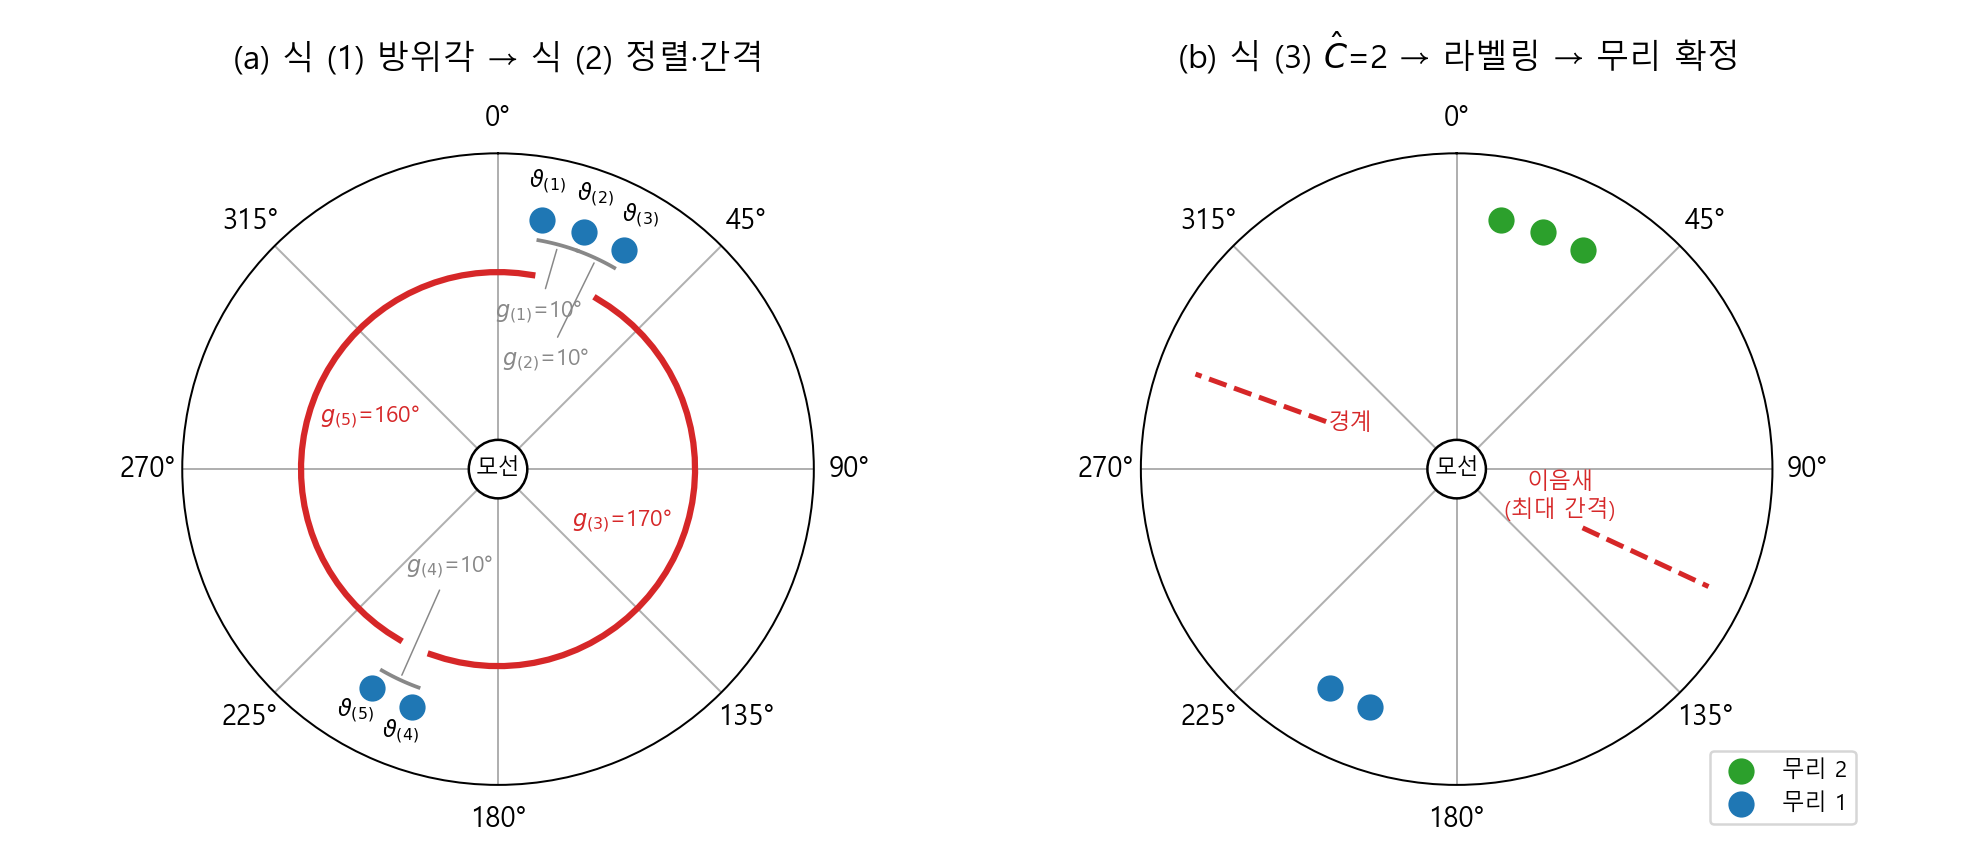
\includegraphics[width=\textwidth]{fig_example1.png}
\caption{(a) 예제의 정렬된 방위와 5개 간격. 빨강이 임계를 넘는 간격. (b) 식~(3)으로 $\hat C=2$, 최대 간격(170°)을 이음새로 열어 라벨링한 결과.}\label{fig:ex1}
\end{figure}

\begin{whybox}[왜 이음새 항이 꼭 필요한가]
북쪽($0^\circ/360^\circ$)에 걸친 무리 때문이다. 방위 $350^\circ, 355^\circ, 5^\circ, 10^\circ$는 실제로 $20^\circ$ 폭의 한 덩어리지만, 정렬하면 $5, 10, 350, 355$가 되어 $10^\circ\!\to\!350^\circ$ 사이에 $340^\circ$짜리 가짜 큰 간격이 생긴다.
이음새 항 $g_{(n)} = 5 + 360 - 355 = 10^\circ$가 있어야 "$355^\circ$와 $5^\circ$는 붙어 있다"는 사실이 수열에 남고, 뒤의 라벨링이 이 둘을 한 무리로 이어 붙인다(그림~\ref{fig:wrap}).
\end{whybox}

\begin{figure}[H]
\centering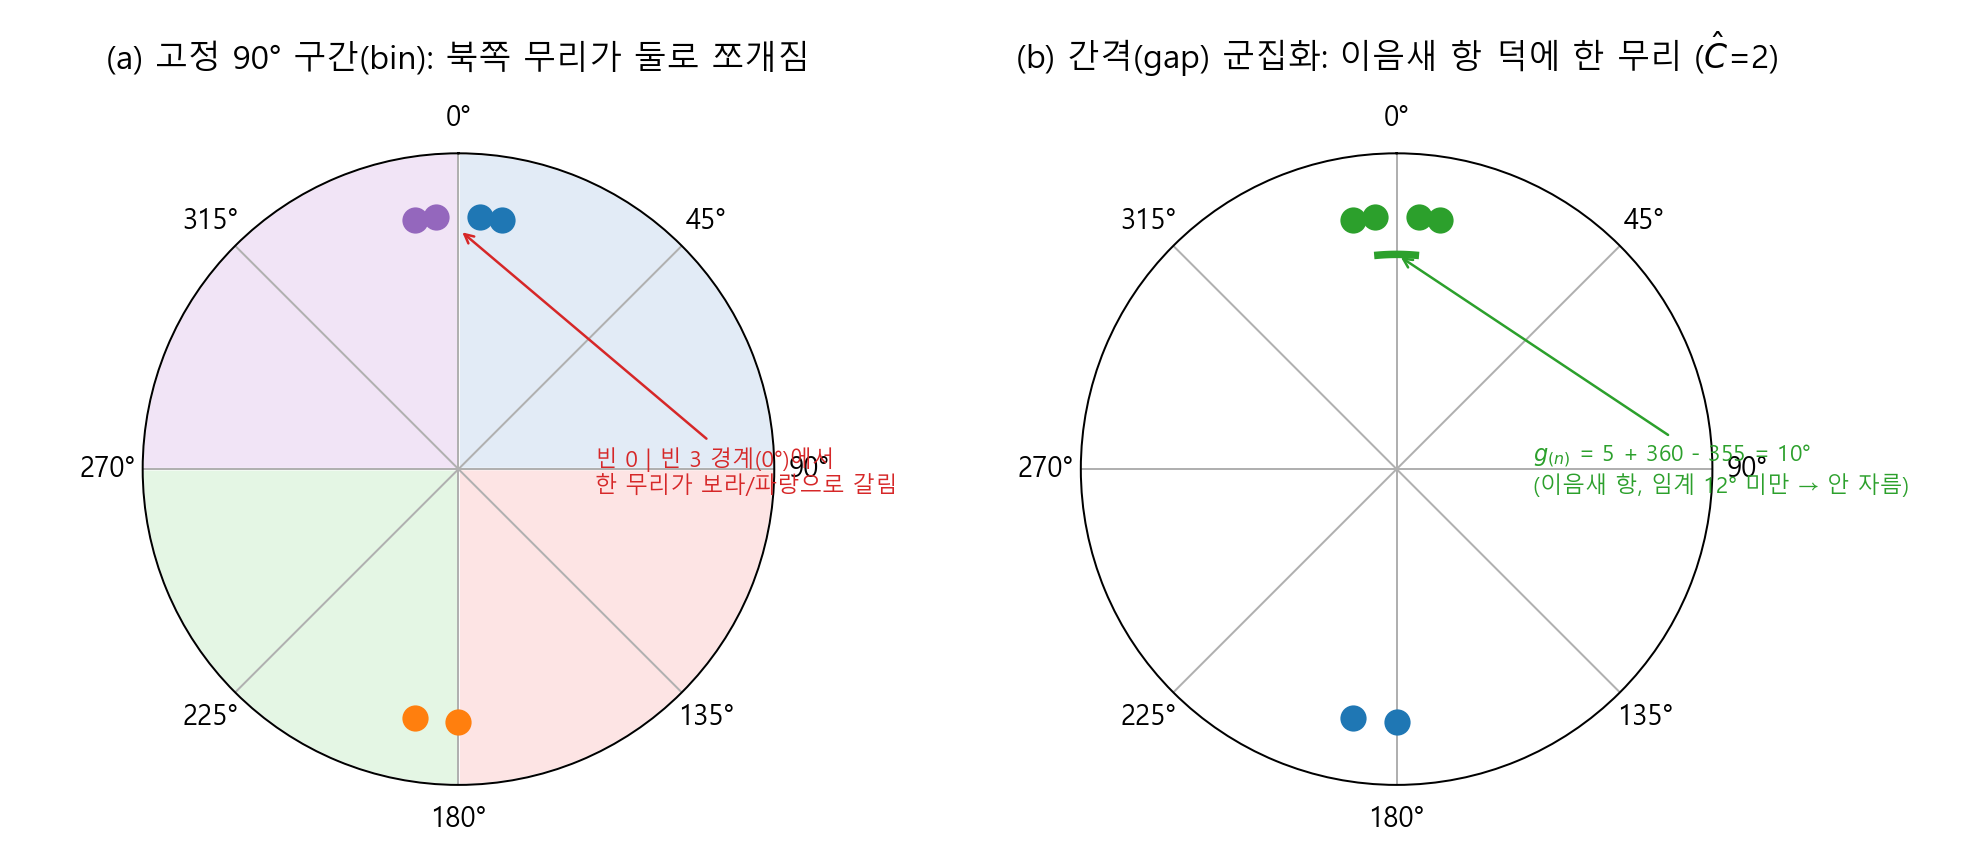
\includegraphics[width=\textwidth]{fig_northwrap.png}
\caption{북쪽에 걸친 무리 $\{350,355,5,10\}$와 남쪽 무리 $\{180,190\}$. (a) 고정 $90^\circ$ 구간 방식은 $0^\circ$ 경계에서 북쪽 무리를 둘로 쪼갠다. (b) 간격 방식은 이음새 항 덕에 한 무리로 유지하고 $\hat C=2$를 얻는다.}\label{fig:wrap}
\end{figure}

\section{식 (3) --- 무리 수}

\begin{equation*}
\hat C = \mathrm{clip}\Big(\big|\{\,q : g_{(q)} > \dgap\,\}\big|,\; 1,\; \min(C,n)\Big) \tag{3}
\end{equation*}

\textbf{무엇을 계산하나.} 무리가 몇 개인지. 안쪽부터 세 겹으로 읽는다.
\begin{enumerate}
\item $\{q : g_{(q)} > \dgap\}$ --- 식~(2)의 간격 중 임계보다 \textbf{큰 것들의 번호 집합}. "이만큼 벌어졌으면 다른 무리"라는 기준.
\item $|\cdot|$ --- 그 집합의 \textbf{원소 수}, 즉 큰 빈틈이 몇 개인가.
\item $\mathrm{clip}(x, 1, \min(C,n))$ --- 아래로 1, 위로 $\min(C,n)$에서 자른다.
\end{enumerate}

\begin{keybox}[원 위에서는 큰 빈틈 k개 = 덩어리 k개]
직선 위에 점을 놓고 큰 빈틈 $k$개에서 자르면 덩어리는 $k+1$개다. 그러나 \textbf{원} 위에서는 마지막 덩어리와 첫 덩어리가 이어져 있으므로 정확히 $k$개가 된다(빈틈 하나가 두 덩어리를 가르는 게 아니라, 빈틈 사이 호(弧) 하나가 덩어리 하나).
이 등식은 이음새 간격 $g_{(n)}$을 세는 것을 전제로 하며, 이것이 식~(2)와 (3)이 짝을 이루는 이유다.
\end{keybox}

\textbf{clip의 두 끝.}
\begin{itemize}
\item 하한 1: 큰 간격이 0개(전부 뭉쳐 있음)여도 무리는 하나 있어야 한다. 실제로 집중 포메이션이 이 경우다.
\item 상한 $\min(C, n)$: 관측 채널이 $C=4$개뿐이고, 적선 $n$척보다 무리가 많을 수는 없다. 상한에 걸리면 뒤의 라벨링이 "가장 큰 $\hat C$개" 간격만 경계로 써서 개수를 맞춘다.
\end{itemize}

\textbf{예제.} 큰 간격은 $170^\circ$($q=3$)와 $160^\circ$($q=5$)의 2개 $\Rightarrow$ $\hat C = \mathrm{clip}(2, 1, \min(4,5)) = 2$.

\begin{whybox}[왜 고정 구간(bin)이 아니라 간격인가]
초기 구현은 $360^\circ/C = 90^\circ$ 고정 구간으로 나눴다(\texttt{clustering.py}의 \texttt{enemy\_clusters\_vec}). 무리가 구간 경계에 걸리면 둘로 쪼개져 요격점이 두 곳으로 흩어지는 아티팩트가 생겼고(그림~\ref{fig:wrap}a), 무리가 하나뿐인 집중 포메이션에서도 빈 구간 3개가 관측에 남았다.
간격 방식은 무리 수를 데이터에 맞춰 $1\sim C$개로 적응시키고, 경계를 데이터가 비어 있는 곳에만 둔다.
\end{whybox}

\begin{whybox}[왜 $\dgap \approx 12^\circ$인가]
파상(wave) 포메이션은 단(rank)마다 방위를 $18^\circ$씩 벌려 생성된다. $\dgap$을 $18^\circ$보다 작게 두면 단마다 별개의 무리가 되어 "시차를 두고 오는 파도"가 무리 수로 드러나고, 같은 단 안의 적선 간 방위차(수 도 이내)보다는 커서 한 단이 쪼개지지 않는다. 그 사이 값으로 12°를 골랐다.
\end{whybox}

\section{(3)과 (4) 사이 --- 누가 어느 무리인가 (라벨링)}

$\hat C$만으로는 식~(4)를 계산할 수 없다. 각 적선 $m$에 무리 번호 $j_m \in \{1,\dots,\hat C\}$를 붙여야 구성원 집합 $\mathcal A_j = \{m : j_m = j\}$가 정해진다. 원고의 문장을 절차로 풀면:
\begin{enumerate}
\item 간격 중 \textbf{가장 큰 $\hat C$개}를 \textbf{경계}로 정한다. (임계와 무관하게 "가장 큰 $\hat C$개"를 쓰므로 clip으로 잘린 경우에도 개수가 맞는다.)
\item 그중 \textbf{최대 간격 하나}를 원의 시작점(\textbf{이음새})으로 연다.
\item 이음새 바로 다음 적선부터 방위 순으로 걸어가며, 경계 간격을 지날 때마다 무리 번호를 $+1$ 한다.
\end{enumerate}
경계 $\hat C$개 중 하나(이음새)는 걷기의 출발점이라 지나지 않으므로, 나머지 $\hat C-1$개를 지나며 번호가 $1$부터 $\hat C$까지 매겨진다.

\textbf{예제.} 경계 = $\{g_{(3)}=170^\circ,\ g_{(5)}=160^\circ\}$, 이음새 = $g_{(3)}$($30^\circ\!\to\!200^\circ$ 사이).
이음새 다음인 $\vt_{(4)}=200^\circ$부터 출발: $200^\circ, 210^\circ$ $\to$ \textbf{무리 1}; 경계 $g_{(5)}$를 지나 $10^\circ, 20^\circ, 30^\circ$ $\to$ \textbf{무리 2}.
원래 번호로 쓰면 $j_1 = j_3 = 1$, $j_2 = j_4 = j_5 = 2$이고 $\mathcal A_1 = \{1, 3\}$, $\mathcal A_2 = \{2, 4, 5\}$ (그림~\ref{fig:ex1}b).

\begin{whybox}[왜 최대 간격을 이음새로 쓰나]
원형 순서에는 "첫 번째"가 없으므로 어디선가 원을 잘라 열어야 한다. 아무 경계나 써도 무리 구성은 같지만, 최대 간격을 고르면 (i) 그것은 반드시 경계이므로 출발점이 무리 한가운데가 되는 일이 없고, (ii) 결정론적이라 같은 배치에서 항상 같은 번호가 나온다. $\hat C=1$이면 경계는 최대 간격 하나뿐이고 걷는 동안 지나지 않으므로 전원이 무리 1이 된다.
\end{whybox}

\section{식 (4) --- 무리 요약 4종}

\begin{equation*}
\begin{aligned}
n_j &= |\mathcal A_j|, \qquad
\bfc_j = \frac{1}{n_j}\sum_{m\in\mathcal A_j}\bfe_m,\\
\Delta\vt_j &= 90^\circ\sqrt{1-\bar R_j}, \qquad
\bar R_j = \Big\lVert \frac{1}{n_j}\sum_{m\in\mathcal A_j}\bhat_m \Big\rVert, \qquad \bhat_m = (\cos\vt_m, \sin\vt_m),\\[2pt]
\vapp_j &= \frac{v_e}{n_j}\sum_{m\in\mathcal A_j}\big\langle(\sin\psi_m, \cos\psi_m),\ \dhat_m\big\rangle, \qquad
\dhat_m = \frac{\bfm-\bfe_m}{\lVert\bfm-\bfe_m\rVert}
\end{aligned} \tag{4}
\end{equation*}

무리 $j$의 구성원 $\mathcal A_j$가 정해졌으니 그것을 네 숫자로 압축한다. 이 네 값이 관측 채널(\S4.4)과 위협도(\S4.3)의 입력이다.

\begin{table}[H]
\centering\small
\caption{네 요약량의 뜻과 용도.}
\begin{tabular}{l l l}
\toprule
기호 & 뜻 & 어디에 쓰이나 \\
\midrule
$n_j$ & 척수 & 휴리스틱 위협도 $\tau_j$(식 5) $+$ 학습 정책 관측 \\
$\bfc_j$ & 무리 중심(위치 평균) & 휴리스틱 위협도·요격점 $\mathbf I_j$(식 5) $+$ 관측 \\
$\Delta\vt_j$ & 각도 퍼짐 & 학습 정책 관측(무리가 방위상 얼마나 넓은가) \\
$\vapp_j$ & 모선 방향 접근 속도 & 학습 정책 관측(얼마나 급한가) \\
\bottomrule
\end{tabular}
\end{table}

\subsection{$n_j$와 $\bfc_j$}

$n_j$는 구성원 수, $\bfc_j$는 구성원 위치의 산술 평균(무게중심)이다. 예제 무리 2($\mathcal A_2=\{2,4,5\}$):
$n_2 = 3$, $\bfc_2 = \frac13\big[(729,4136)+(2200,3811)+(1368,3759)\big] = (1432,\ 3902)$ m.

\subsection{$\Delta\vt_j$ --- 각도 퍼짐: 왜 표준편차를 안 쓰나}

\textbf{문제.} 각도는 원 위의 양이라 산술 평균·표준편차가 깨진다. $350^\circ$와 $10^\circ$의 실제 차이는 $20^\circ$인데 산술 평균은 $180^\circ$, 편차는 $170^\circ$로 나온다(wrap 문제).

\textbf{해법: 원형 통계의 결집도(mean resultant length).}
\begin{enumerate}
\item 각 방위를 \textbf{단위벡터} $\bhat_m = (\cos\vt_m, \sin\vt_m)$로 바꾼다. 원 위의 점을 좌표로 옮기는 것이므로 wrap 문제가 사라진다.
\item 벡터들을 \textbf{평균}하고 그 \textbf{길이} $\bar R_j$를 잰다.
  \begin{itemize}
  \item 모두 같은 방향 $\Rightarrow$ 벡터가 겹쳐 길이 $\mathbf 1$.
  \item 사방으로 흩어짐 $\Rightarrow$ 서로 상쇄돼 길이 $\mathbf 0$.
  \end{itemize}
\item $1-\bar R_j$가 \textbf{원형 분산}(circular variance)이다. 제곱근을 취해 "표준편차 꼴"로 만들고 $90^\circ$를 곱해 각도 단위로 맞춘다.
\end{enumerate}

\begin{figure}[H]
\centering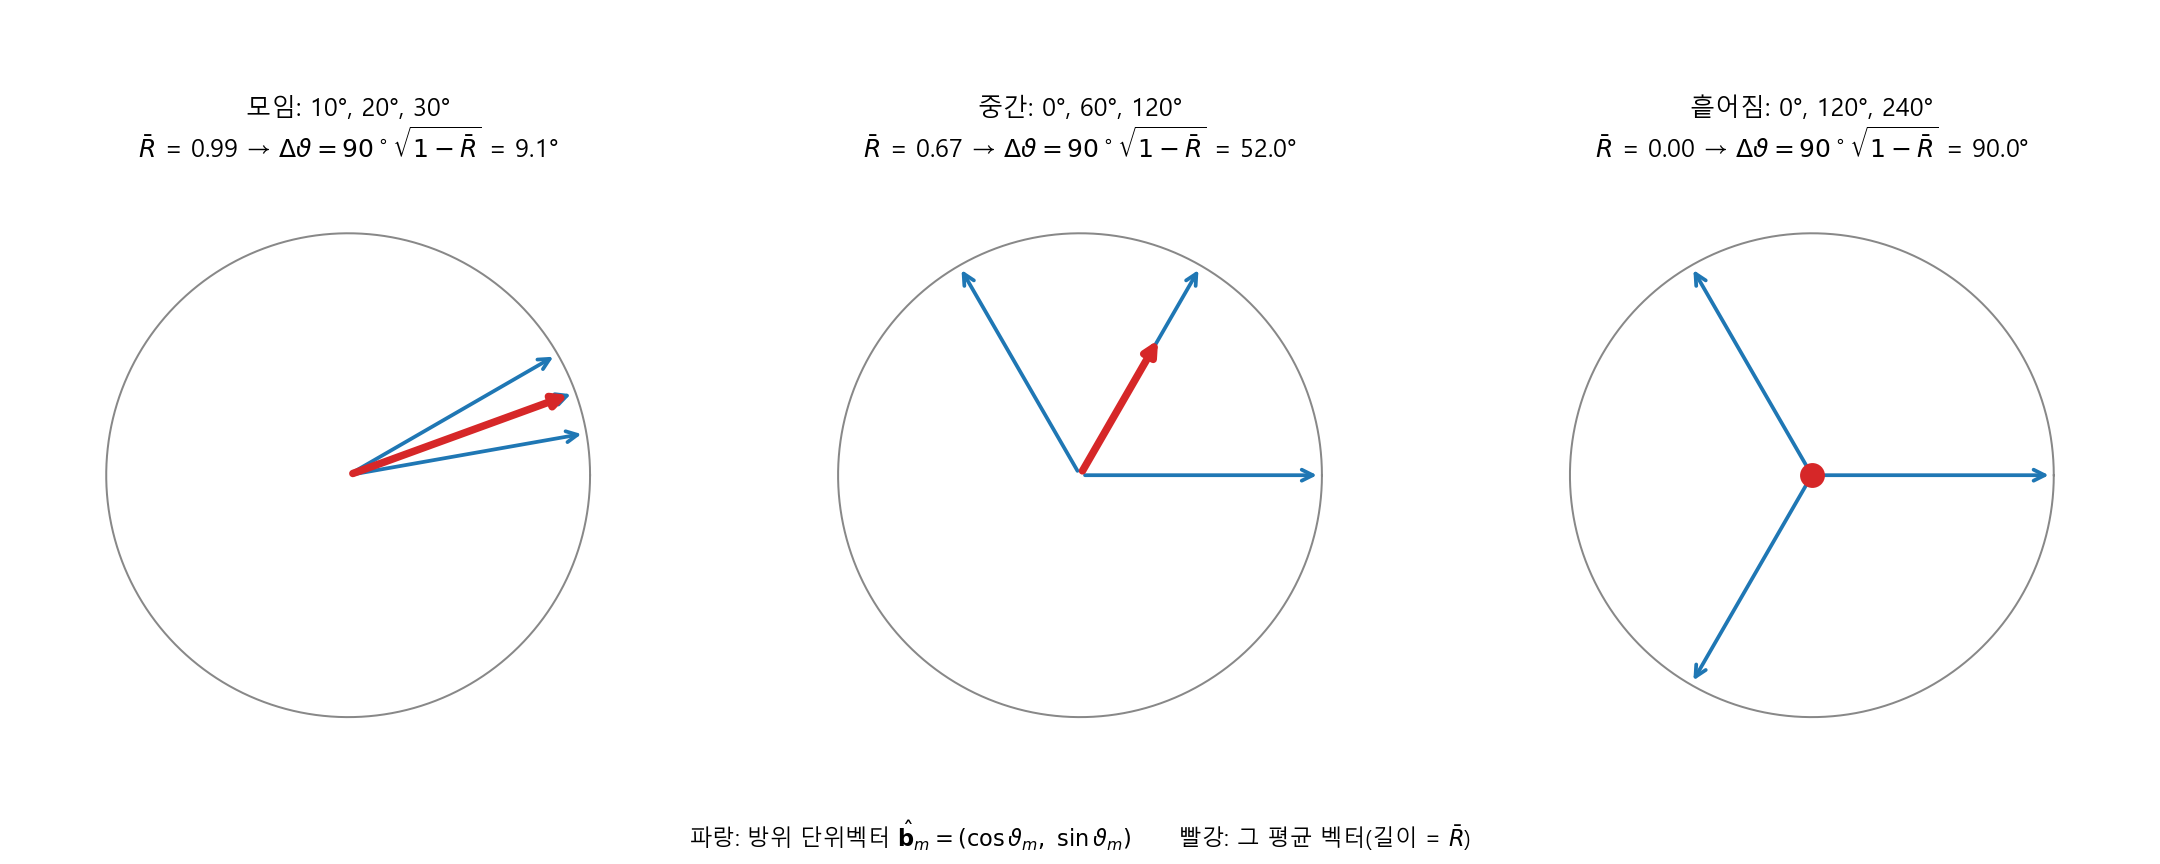
\includegraphics[width=\textwidth]{fig_resultant.png}
\caption{결집도 $\bar R$의 기하. 파란 단위벡터들의 평균(빨강)이 길수록 방위가 모여 있다.}
\end{figure}

\begin{whybox}[왜 90도를 곱하나]
두 가지 근거가 겹친다. (i) \textbf{상한}: $\bar R=0$(완전 분산)에서 $\Delta\vt = 90^\circ$, $\bar R=1$에서 $0^\circ$로 범위가 $[0^\circ, 90^\circ]$에 깔끔히 갇힌다. (ii) \textbf{소각 근사}: 방위가 표준편차 $\sigma$(라디안)로 모여 있으면 $\bar R \approx 1 - \sigma^2/2$이므로 $\sigma \approx \sqrt{2(1-\bar R)}$, 도 단위로 $\frac{180}{\pi}\sqrt2\,\sqrt{1-\bar R} \approx 81^\circ\sqrt{1-\bar R}$. 즉 $90^\circ$는 실제 각도 표준편차에 가까운 스케일이다. 예제 무리 2($10,20,30^\circ$)는 산술 표준편차 $8.2^\circ$, 식~(4)로 $9.1^\circ$.
\end{whybox}

\textbf{예제 무리 1}($200^\circ, 210^\circ$):
$\frac12(\cos 200^\circ + \cos 210^\circ) = -0.903$, $\frac12(\sin 200^\circ + \sin 210^\circ) = -0.421$,
$\bar R_1 = \sqrt{0.903^2 + 0.421^2} = 0.996$, $\Delta\vt_1 = 90^\circ\sqrt{1-0.996} = 5.6^\circ$.

\textbf{참고.} $\bhat_m$은 $\bar R$ 계산에만 쓰이므로 $(\cos,\sin)$ 순서(수학 규약)여도 무방하다. 길이는 축을 어떻게 잡든 같다.

\subsection{$\vapp_j$ --- 접근 속도: 침로와 모선 방향의 내적}

\textbf{문제.} 같은 거리에 있어도 모선을 향해 오는 무리와 옆으로 지나가는 무리는 위협이 다르다. 속력 $v_e$ 중 \textbf{모선 쪽 성분}만 뽑고 싶다.

\textbf{구성 요소.}
\begin{itemize}
\item $\psi_m$: 적선 $m$의 \textbf{침로}(heading). 항법 규약이므로 침로 단위벡터의 (동, 북) 성분은 $(\sin\psi_m, \cos\psi_m)$이다(표~\ref{tab:conv}). 수학 규약의 $(\cos, \sin)$과 자리가 바뀐 이유가 이것이다.
\item $\dhat_m$: \textbf{적선에서 모선을 향하는 단위벡터}.
\item $\langle\cdot,\cdot\rangle$: 두 단위벡터의 내적 $=$ 두 방향 사이 각의 $\cos$. 정면으로 모선을 향하면 $+1$, 옆으로 스치면 $0$, 멀어지면 음수.
\item $v_e$: 적선 속력. 내적에 곱하면 "모선 쪽으로 다가오는 속도 성분"이 된다. 무리 전체로 평균.
\end{itemize}

\begin{figure}[H]
\centering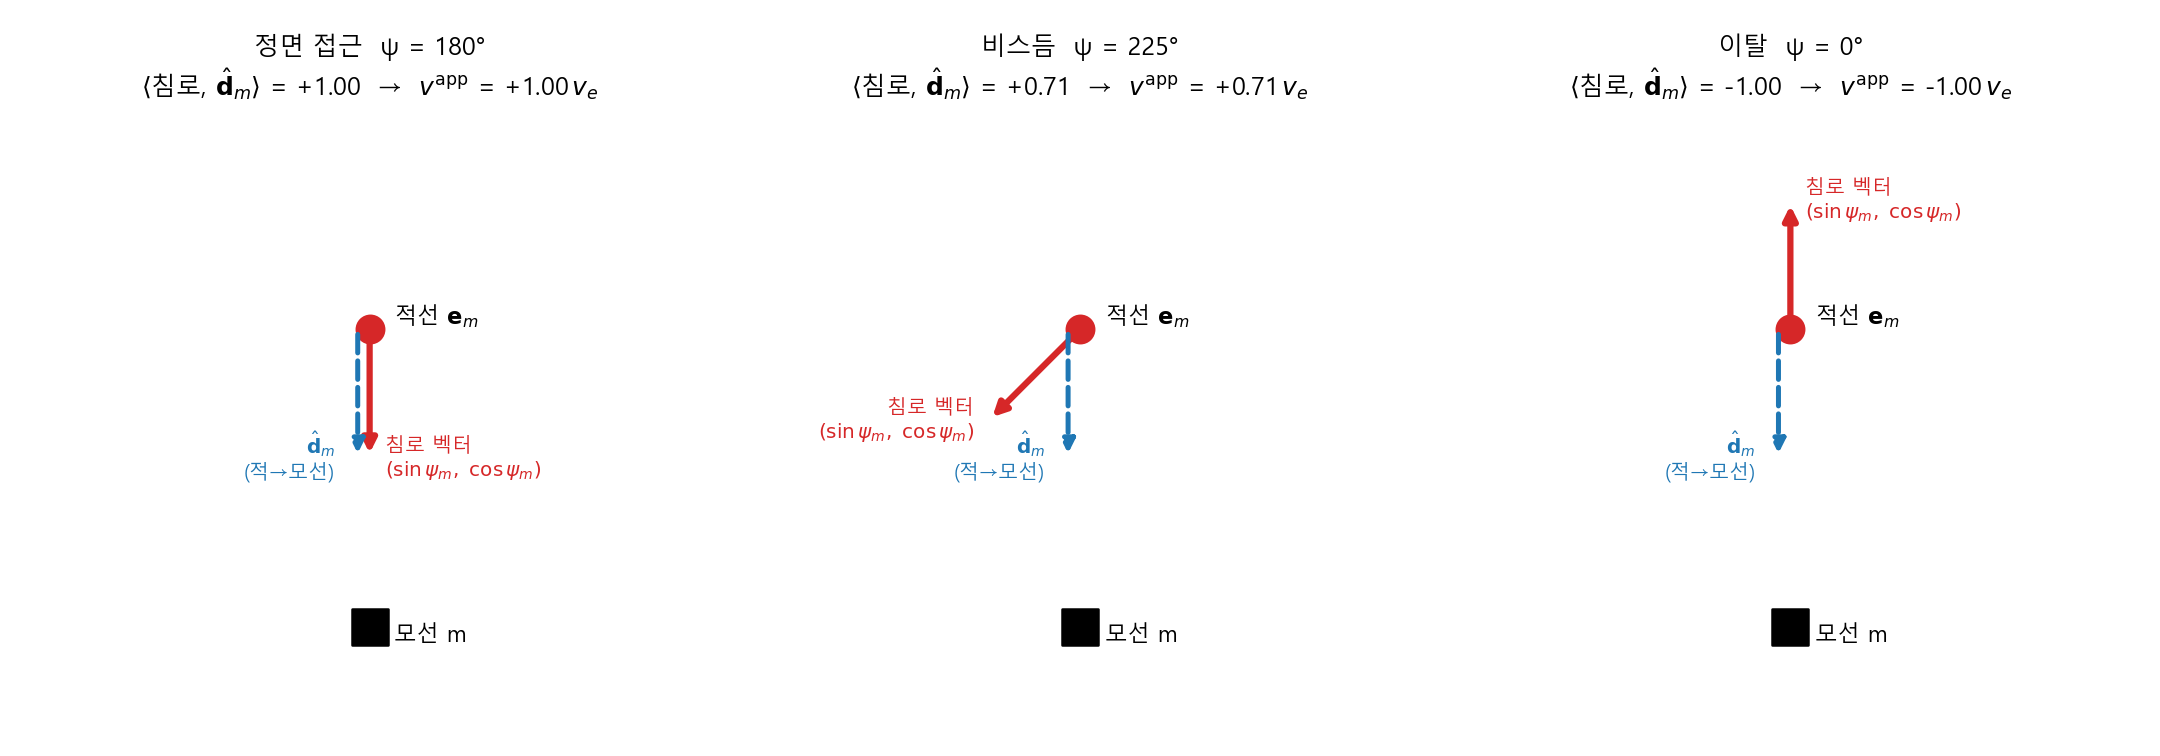
\includegraphics[width=\textwidth]{fig_approach.png}
\caption{침로 벡터(빨강)와 모선 방향 벡터(파랑 점선)의 내적. 적선이 모선 정북 3 km에 있을 때 침로별 접근 속도.}
\end{figure}

\textbf{예제 무리 1.} 적선 1: 방위 $200^\circ$, 침로 $20^\circ$ $\Rightarrow$ 정확히 모선을 향함, 내적 $1.000$. 적선 3: 방위 $210^\circ$, 침로 $60^\circ$ $\Rightarrow$ 모선 방향($30^\circ$)에서 $30^\circ$ 벗어남, 내적 $\cos 30^\circ = 0.866$.
$\vapp_1 = \frac{10}{2}(1.000 + 0.866) = 9.33$ m/s.

\section{예제 최종 결과}

\begin{table}[H]
\centering\small
\caption{예제 5척의 군집화 결과 (관측 채널에 들어가는 값).}
\begin{tabular}{c c c c c c}
\toprule
무리 $j$ & 구성원 $\mathcal A_j$ & $n_j$ & $\bfc_j$ (m) & $\Delta\vt_j$ & $\vapp_j$ (m/s) \\
\midrule
1 & $\{1, 3\}$ (200°, 210°) & 2 & $(-2155,\,-4601)$ & $5.6^\circ$ & $9.33$ \\
2 & $\{2, 4, 5\}$ (10°, 20°, 30°) & 3 & $(1432,\,3902)$ & $9.1^\circ$ & $9.99$ \\
3, 4 & --- (비활성) & 0 & --- & --- & --- \\
\bottomrule
\end{tabular}
\end{table}
$C=4$이므로 채널 3, 4는 비어 있고, 관측에서는 "활성" 플래그 0으로 표시된다.
휴리스틱 위협도 $\tau_j = n_j\cdot\mathrm{clip}(1-\lVert\bfc_j-\bfm\rVert/R_w,\,0.05,\,1)$(식~5)는 척수와 근접도만 쓰므로, 척수가 많고 더 가까운($\approx$4.2 km) 무리 2가 먼저 배정된다. $\Delta\vt_j$와 $\vapp_j$는 학습 정책의 관측 벡터로 들어가 정책이 스스로 가중치를 배운다(구현: \texttt{defense\_env.py}의 \texttt{enemy} 관측, 각각 \texttt{spread\_norm}과 $/v_e$로 정규화).

\section{자주 헷갈리는 점 정리}

\begin{table}[H]
\centering\small
\begin{tabular}{p{0.34\textwidth} p{0.6\textwidth}}
\toprule
질문 & 답 \\
\midrule
$\vt_m$과 $\vt_{(q)}$의 차이? & $m$은 적선 번호, $(q)$는 정렬 후 순번. 같은 값들을 다른 순서로 부른 것. \\
$g_{(q)}$와 $g_{(n)}$은 다른 양인가? & 아니다. 같은 수열의 일반항과 마지막 항. 마지막만 원을 돌아와야 해서 식이 따로 쓰였다. \\
빈틈 개수가 곧 무리 수인 이유? & 원 위에서는 빈틈 $k$개 사이의 호 $k$개가 곧 덩어리. 이음새 항을 세야 성립. \\
큰 간격이 $\hat C$보다 많으면? & clip 상한에 걸림. 라벨링은 "가장 큰 $\hat C$개"만 경계로 쓰므로 나머지 큰 간격은 무시되고 이웃 무리가 합쳐진다. \\
$\Delta\vt$에 왜 $\cos/\sin$이 나오나? & 각도를 원 위 좌표로 바꿔 평균하기 위해. 각도의 산술 평균은 $0/360$ 경계에서 틀린다. \\
$\vapp$에 왜 $(\sin\psi, \cos\psi)$인가? & 북쪽 $0^\circ$·시계 규약에서 침로의 (동, 북) 성분. $(\cos,\sin)$은 동쪽 $0^\circ$ 규약. \\
$\vapp$이 음수면? & 무리가 평균적으로 멀어지는 중. 관측값 $\vapp/v_e \in [-1, 1]$이 음수로 들어가 정책이 급하지 않은 무리로 학습한다. \\
\bottomrule
\end{tabular}
\end{table}

\appendix
\section{원고 식 $\leftrightarrow$ 구현 코드 대응}

구현은 \texttt{boatattack\_sim/env/clustering.py}의 \texttt{cluster\_by\_gaps\_vec}이며 $N$개 월드를 벡터화한 것 외에는 원고와 1:1이다.
\begin{table}[H]
\footnotesize
\begin{tabularx}{\textwidth}{>{\raggedright\arraybackslash}p{0.2\textwidth} >{\raggedright\arraybackslash}X >{\raggedright\arraybackslash}p{0.19\textwidth}}
\toprule
원고 & 코드 (줄) & 비고 \\
\midrule
식 (1) $\operatorname{atan2}(\Delta x,\Delta y) \bmod 360$ & \texttt{np.degrees(np.arctan2(dx, dy)) \% 360.0} (100) & Python \texttt{\%}는 $[0,360)$ 보장 \\
식 (2) $g_{(q)},\ q<n$ & \texttt{cg = sb[:,1:] - sb[:,:-1]} (110) & \texttt{sb} = 정렬된 방위 \\
식 (2) $g_{(n)}$ 이음새 & \texttt{wrap = sb[:,0] + 360.0 - last} (116) & \\
식 (3) clip & \texttt{B = np.clip((gaps > gap\_deg).sum(1), 1, K)} (120); \texttt{B = np.minimum(B, cnt\_alive)} (121) & 상한 $\min(C,n)$ \\
라벨링: 이음새 & \texttt{seam = desc[:,0]} (129) & 최대 간격 위치 \\
라벨링: 경계 통과 시 $+1$ & \texttt{cur = cur + boundary[...]} (140) & \\
식 (4) $\bfc_j$ & \texttt{cent[:,k,0] = (e\_pos * m).sum(1) / den} (163) & \\
식 (4) $\bar R_j$, $\Delta\vt_j$ & \texttt{R = np.hypot(cosb, sinb)}; \texttt{sqrt(1-R)*90} (167--168) & \\
식 (4) $\vapp_j$ & \texttt{evx = sin(hdg)*speed}; \texttt{(evx*emx+evy*emy)/emn} (150--154) & \texttt{emn} $=\lVert\bfm-\bfe_m\rVert$ \\
$C=4$, $\dgap$ & \texttt{config.py}: \texttt{n\_clusters=4} (315), \texttt{cluster\_gap\_deg=11.97} (338) & \\
\bottomrule
\end{tabularx}
\end{table}

\end{document}
